\documentclass[border=0pt]{standalone}
\usepackage{tikz}
\usetikzlibrary{positioning,shapes,arrows.meta,patterns,calc}
\definecolor{garnet}{HTML}{73000A}
\definecolor{coral}{HTML}{CC2E40}
\definecolor{slate}{HTML}{466A9F}
\definecolor{teal}{HTML}{1F414D}
\definecolor{olive}{HTML}{65780B}
\definecolor{lime}{HTML}{CED318}
\definecolor{gold}{HTML}{A49137}
\begin{document}
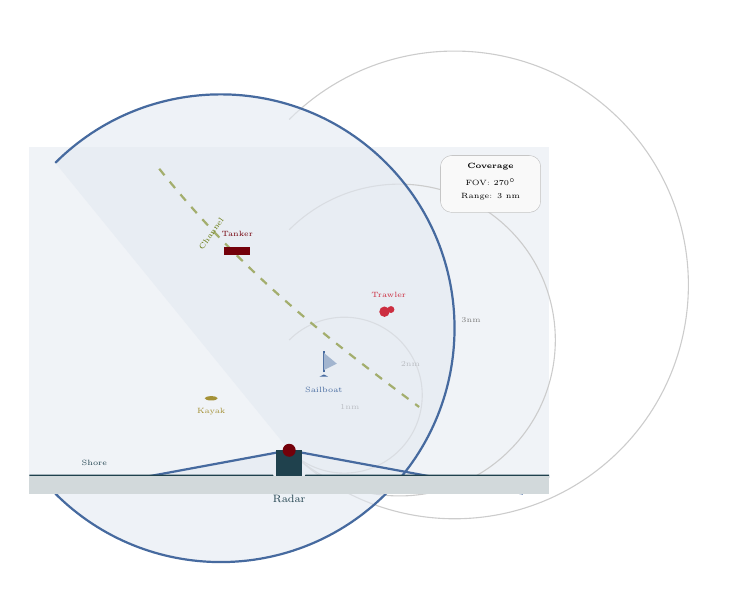
\begin{tikzpicture}[scale=0.55, transform shape]
    % Sea background with gradient effect
    \fill[slate!8] (-6,-1) rectangle (6,7);
    
    % Range rings
    \foreach \r/\label in {1.8/1nm, 3.6/2nm, 5.4/3nm} {
        \draw[gray!40, thin] (0,0) arc[start angle=-135, end angle=135, radius=\r];
    }
    % Range labels
    \node[font=\tiny, gray] at (1.4,1.0) {1nm};
    \node[font=\tiny, gray] at (2.8,2.0) {2nm};
    \node[font=\tiny, gray] at (4.2,3.0) {3nm};
    
    % Coverage arc (270 degrees) - filled wedge
    \fill[slate!15, opacity=0.6] (0,0) -- (-5.4,-1) arc[start angle=-135, end angle=135, radius=5.4] -- cycle;
    \draw[slate, thick] (0,0) -- (-5.4,-1);
    \draw[slate, thick] (0,0) -- (5.4,-1);
    \draw[slate, thick] (-5.4,-1) arc[start angle=-135, end angle=135, radius=5.4];
    
    % Radar position (shore)
    \fill[teal] (-0.3,-0.8) rectangle (0.3,0);
    \fill[garnet] (0,0) circle (0.15);
    \node[below, font=\scriptsize, teal] at (0,-0.9) {Radar};
    
    % Shore line
    \draw[teal, very thick] (-6,-0.6) -- (-0.4,-0.6) -- (-0.3,-0.8);
    \draw[teal, very thick] (0.3,-0.8) -- (0.4,-0.6) -- (6,-0.6);
    \fill[teal!20] (-6,-1) rectangle (6,-0.6);
    \node[font=\tiny, teal] at (-4.5,-0.3) {Shore};
    
    % Shipping channel
    \draw[olive!60, dashed, thick] (-3,6.5) .. controls (-1,4) and (1,2.5) .. (3,1);
    \node[font=\tiny, olive, rotate=55] at (-1.8,5) {Channel};
    
    % Vessels at different ranges
    % Container ship (far)
    \fill[garnet] (-1.5,4.5) rectangle (-0.9,4.7);
    \node[font=\tiny, garnet] at (-1.2,5.0) {Tanker};
    
    % Fishing boat (mid)
    \fill[coral] (2.2,3.2) circle (0.12);
    \fill[coral] (2.35,3.25) circle (0.08);
    \node[font=\tiny, coral] at (2.3,3.6) {Trawler};
    
    % Sailboat (near)
    \draw[slate, thick] (0.8,1.8) -- (0.8,2.3);
    \fill[slate] (0.7,1.7) -- (0.9,1.7) -- (0.8,1.75) -- cycle;
    \fill[slate!50] (0.8,1.85) -- (0.8,2.25) -- (1.1,2.0) -- cycle;
    \node[font=\tiny, slate] at (0.8,1.4) {Sailboat};
    
    % Kayak (very near)
    \fill[gold] (-1.8,1.2) ellipse (0.15 and 0.05);
    \node[font=\tiny, gold] at (-1.8,0.9) {Kayak};
    
    % Legend box
    \draw[gray!50, rounded corners] (3.5,5.5) rectangle (5.8,6.8);
    \fill[gray!5, rounded corners] (3.5,5.5) rectangle (5.8,6.8);
    \node[font=\tiny\bfseries] at (4.65,6.55) {Coverage};
    \node[font=\tiny] at (4.65,6.2) {FOV: 270$^\circ$};
    \node[font=\tiny] at (4.65,5.85) {Range: 3~nm};
\end{tikzpicture}
\end{document}
